\chapter{Acquisition of non-stationary impedance}
% \minitoc
\label{ch:acquisition}

This work gives a complete chain for the measurementes of dynamic ipedance spectroscopy:
\begin{itemize}
    \item design and generation of the excitation signal
    \item acquisition of multi-frequency signals with automated set-up
    \item estimation of istantanous impedance from multi-frequency voltage and current signals
    \item analysis of the impedance data for characterization of cells and surface processes
\end{itemize}
This chapter deals with the firs two points \dots

% Introduction and motivation

% Limitation of classical EIS
Electrochemical impedance measurement is traditionally performed under the assumption of stationarity. Its validity vanishes whenever the internal state of the system evolves on comparable or shorter timescales; as occurs during battery charge and discharge, SEI formation, lithiation-induced expansion, or any experiment where the current is not zero for long enough to reach equilibrium.

% Need for broadband, time-resolved measurements
While impedance has been measured in electrochemical storage devices, it was either limited to frequency higher of 1Hz or multisine spanning only 3-4 decades. A full broadband spectra for batteires requires to experiment to be interrupted and waiting for the stationarity condition, which adds overheading time to the battery test making impedance impractical to use in operando conditions.

% Overview of the methodology
This chapter describes the practical methodology and instrumental chain developed to acquire \emph{non-stationary} impedance, i.e. the time-resolved evolution of impedance over several decades of frequency while the system is drifting due to the imposed load. The goal is to obtain continuous impedance spectra over seven orders of magnitude in frequency without interrupting the charge/discharge process.

The principle of the set-up follows the classical design from the literature. A multisine of small amplitude is superimposed to a high-amplitude drift and applied to the cell though a potentiostat. The voltage and current analog signals are sampled at high frequency by a dedicated acquisition device and streamed to a computer. Impedance is estimated from the fouerire trasnform of voltage and current at the frequencies components $\omega_i$ of the multisine excitation. 

The novelty of this work is a methodology that combines the ST-FFT and DMFA to compute the istantanous time-resolved impedance. The first method is used online for the high frequency band and it is followed by a strong downsample, while the secon is applied off-line. The result of the two methods is concatenated to obtain to complete bradband time-resolved spectra.

The methodology combines:
\begin{itemize}
    \item frequency-optimized multisine excitation,
    \item synchronized high-frequency digitization,
    \item real-time spectral estimation and segmentation,
    \item hardware-aware design (memory limits, ADC resolution, synchrony, jitter),
    \item and a Python-based automation framework (called DEIStools) for coordinating potentiostat, waveform generator and oscilloscope.
\end{itemize}

The chapter is organized as follows: 
\begin{itemize}
    \item [\textbf{Section~\ref{sec:hardware}}] describes the experimental hardware chain;
    \item [\textbf{Section~\ref{sec:multisine}}] details the generation, splitting and  optimization of multisine waveforms; 
    \item [\textbf{Section~\ref{sec:sampling}}] addresses sampling, synchronization and spectral leakage;  
    \item [\textbf{Section~\ref{sec:automation}}] summarizes the automation architecture;  
    \item [\textbf{Section~\ref{sec:designrules}}] provides practical guidelines and limitations.
\end{itemize} 

The method for estimating the impedance from multi-frequency data will be the topic of next chapter.

\section{Hardware}
\label{sec:hardware}

% Potentiostat (also intenral architecture?)
% AWG
% Oscilloscope / ADC
% Cabling and isolation
The instrumental set-up used in our labs follows the same design introduced  in section \ref{sec:fft-eis} with a potentiostat interfaced with a dedicated waveform generator, for the excitation, and a dedicate acquisition device for high-frequency sampling and streaming to a computer. 
The multisine excatation is generated as analog voltage signal and injected into the potentiostat where it is superimposed on the main drift. 
It is converted to current though the measurement resistor when the tehnique applied by the potentiostat is galvanostatic.

For this work we assembled multiple set-ups using BioLogic potentiostats, Keysight waveform generators and PicoTech Picoscope acquisition devices. 
The components are connected together using the auxiliary input-output port of the potentiostat: the waveform generator to the input and the scope recieves the voltage and current signals for the synchronous sampling. 
The series and the model might vary experiment by experiment, therefore I will report the exact devices in the next part of the thesis where the results of discussion of multiple application of DEIS are reported. 
The brand, though, remain the same as well as the operating principles and they can be all used with the software solution developed here. 
BioLogic potentiostats have for each channel an auxiliary 9-pin port for the input and output of analog signals. 
For the purpose of this project I was interested in only three: Input (Auciliary In2), voltage monitor and current monitor. The company supplies adapters for the 9-pin to BNC connectors but for me was more practical to build them myself with my requirments. 
A reference for the contruction is available in the Appendix \ref{ap:aux cable}.

\section{Multi-sine design}
\label{sec:multisine}
A multisine is the superposition of many sinusoidal components:
\[
u(t) = \sum_{k=1}^{K} A_k \sin(j2\pi f_k t + \phi_k).
\]
It allows the simultaneous excitation of a large set of frequencies with a 
single time-domain waveform, dramatically reducing the experiment duration.

Obtaining high-quality non-stationary impedance, however, requires careful design of the multisine: frequency grid, crest-factor minimization, amplitude choice and memory constraints of the AWG.

\subsection{Frequencies selection}

The frequencies f must be chosen in a way that one period of the whole multi-sine contains integer numbers of oscillation to ovoid spectral leakage. 
The period is then defined by one oscillation of the sinus with lowest frequency $T=\frac{1}{f_{min}}$.
Every other frequency i-th must satisfy the condition $f_i=k\times f_{min}$, where k is an integer. 
In this work we generate the desired frequencies from an harmonic series of integer to insure the above condition and the possibility to re-use the sequence for multi-sine with different $f_{min}$. 
With the term harmonic sequence I refer to $h_i =\frac{f_i}{f_{min}}$; such that it always starts from 1. The sequence is generated as a logarithmic distribution with a number of point per decade between six and ten; I generally obtain good densities with 8 ponints per decade. 
Lower values gives spares spectra while high values give a denser one. 
Denser spectra are more beneficial for the data regression having more points to cast in the cost function, but the power of the signal increases. 
Eight points seems to me the sweet spots, according to my experience.

\subsection{Amplitude optimization}
\label{sec:amplitude optim}
When the amplitudes are all the same, it is said to have a "flat" multi-sine. 
To question is: how to decide the amplitudes?  It can be achieved via analytical formulas or experimental extrapolation. 
The first case was used in Battistel and Hellemans, with opposite results, making the amplitudes drop logarithmically with the increase of the frequency.  
In my work, I measured the non-stationary impedance for many different chemistry and geometries obtaining quite different results in sense of the module of the impedance. 
Hence, I prefer the approach of choosing the amplitudes based on previous experiment. 
One can just measure a classic stepped-sine impedance with any electrochemical workstation and use its module to calculate the desired input amplitude. 
Alternatively, and more effective for energy storage systems, is to measure the non-stationary impedance firs using a flat multi-sine and then extract from the, often noisy, data the average value and use again its module.
% Moved from the other chapter
Firstly I measured a complete cycle of the battery with dynamic impedance spectroscopy using a equal amplitudes on a test cell (not part of the dataset), and then I used the avarage of the module of such impednace and used it to calculate the amplitudes for the input in order to obtain an output with equal magnitude for each frequencies. 
In mathematical therms, being $|Z_{test}(\omega)|_{avg}$ the avarege of the impedance module, the desired output voltage is unitary for all frequencies, enche the current amplitude follows Ohm's law as:

$$
i(\omega_k) = \frac{1}{|Z_{test}(\omega_k)|_{avg}}.
$$

The output of the waveform generator is a voltage and it is converted to current by the electrochemical workstation during the chronoamperometry technique using the active measurement resistor ($R_m$). 
For this experiments I choose always the same current range of 10 mA for the sequence that translates to a measurement resistor of 100 Ohms. 
Hence for the galvanostatic step the actual peak-to-peak voltage of the generated waveform is 

$$
V(\omega_k) = R_m \times i(\omega_k).
$$

For the potentiostatic step instead the amplitude of the multisine is 

$$
V(\omega_k) = |Z_{test}(\omega_k)|_{avg}.
$$

\subsection{Phase optimization}
The process of identification should be carried out with small amplitude excitation around the operating point point. 
Multi-sine waveforms can often time have large peak to peak total amplitude after optimizing the relative amplitudes derives by the superimposition of multiple sinusoidal component at the value of their peak. 
In most cases though, it can be reduced acting on the phase of each sinusoidal component in the total multisine. 
The quantity one is interested to reduce is the \textit{crest factor} (CF) defined as

$$
CF = \frac{|x_{max}|}{x_{rms}}
$$

where $x_{rms}$ is the root-mean-square and consequently the peak-to-average power factor (PAPR) equal to the square of the crest factor. 
The crest factor of a pure sinusoidal wave if $\sqrt{2}$ that serves as a lower ideal boundary  (it is matched only by a chirp waveform, a square wave though as a CF of 1). 
The crest factor minimization consist of solving the optimization problem

$$
\min _\theta 
$$

Multiple approaches has been proposed in the field and their characteristic is a trade-off between speed and accuracy (find the absolute minimum). 
The right method strongly depends on the type of problem and on the following characteristics: distribution of frequency (logarithmic or linear), number of points per decades, number of frequencies in the waveform and relative amplitude (flat, linear, logarithmic, arbitrary). 
A summary of the main method for crest-factor minimization are described in the Appendix \ref{ch:crest factor}. 
In this work, the iterative-stochastic optimization was used in all the experiments presented later, although not the optimal it gives a sufficiently low CF for the explorative stage of this work.

\subsection{Multisine design library}

To streamline the design of multisines I created a Python library also for it, with the name Multisine. 
It provides the object Multisine that generates multisine, optionally optimize phases for minimal crest factor though iterative randomization and provides tools for visual spectral analysis. 
It is available as open source software at XXX.github

\subsection{AWG memory limitations and splitting strategy}
\label{sec:multisine split}
Benchtop Waveform generators consist of electronic circuits made around a digital-to-analog converter (DAC).
An integrated modern DAC chip has a buffer memory in which the waveform values are written and during the generation such memory is read in loop.  
Commercial devices have a buffer memory consisting of 12 to 32 kSa that is quite small for the excitations used in batteries that might span 6-7 decades (at least for the laboratory scale). 
A practical solution (used for example for the playback of audio files in any electronic device) is called direct digital synthesis (DDS) that creates a direct communication between a DAC and a micro-controller with sufficient memory. 
This option require to be proficient in the programming and setting of micro-controller, specifically synchronizing the parts to the same clock. 
In our laboratory we use instead a dedicated bench-top Arbitrary Waveform Generator (AWG) with two channels each with 64MSa; a huge upgrade to conventional integrated DACs. 
This amount of memory allow multi-sine waveforms containing at least 6 decades. 
It is, in fact, the standard device use in the set-ups for dynamic impedance available in the laboratory.
 Indeed, most of the experiments described later use one channel of the generator for the multi-sine perturbation. 

To study batteries, though, my desire was to have seven or more decades in the multi-sine and being able to switch between two waveforms optimized specifically for a chronopotentiometry and a chronoamperometry. 
The solution I came up with is to divide a multi-sine waveform into two waveforms and use the ability of the generator to sum the signals of the two channels ( "dual channel mode") at output.  
The two separate waves are much 'shorter' in  'lenth of samples' and allow to fit two types of multisines in the memory of the device. 
Let's consider a seven-decade multisine waveform from 10mHz to 100kHz, generated at 1MHz (the higher the frequency, the lower is the leakage that will be brought into the FFT of the signal. 
Using 10 times the value of the maxium frequency is giving us good results; some advice even to use 100 times. 
It might be also depending on the method the device uses for generation. 
Keysight devices have a proprietary 'TrueForm' technology to reduce jitter that might help with limiting the spectral leakage in the final signal).  
Generating it in one waveform correspond to 100 MSa (obtained as $period \times f_{gen}$). 
Dividing (or splitting) the wave at the middle frequency of 100Hz creates two waves: one from 10mHz to, around, 100Hz (the frequency before in the list) generated at 1000Hz of length 100kSa and a second one from exactly 100Hz to 100kHz generated a 1mHz that, chosing a period of 1s, leads to a waveform of 100kSa. 
The two will take up only 200kSa of the generator memory to produce the same excitation.

In the example I used two arbitrary parameters: the 100Hz boundary frequency and the 1s period of the high band waveform. 
For my case 100Hz sits in the middle so this might be adjusted case by case with the same rationale. 
Regarding the period of the second wave, one might think of using 0.01 second to have one exact period of the lowest frequency. 
One must now consider that the frequencies of the two waves must follow the same rules described before to avoid intermodulation and such, being made from a sequence of harmonics. 
Logarithmic sequences chosen for intermodulation tend to be sparser on the low frequency part and denser later. 
If for both waveform one generates the frequencies start from the harmonic of 1, the measured impedance spectra would have a sparser points distribution in the decade from 100Hz and 1kHz where the  high band multi-sine waveform starts. 
To get a uniform distibution of points, I generated the frequencies starting from 1 Hz and discarded the points until 100Hz (not included), since they are already presnet in the low band waveform. 
Then, the period of the waveform must be of 1Hz otherwise there will be spectral leakage in the final excitation (note that the frequencies are all integer multiples of 1Hz). 
The sum of the two smaller waveforms generated with this method have the exact distribution of a signle-gnerated wave. 
Figure \ref{fig:splitting_design} shows the density of points when restarting the multisine from 100Hz, from 10 Hz and discarding the first decade and 1 Hz and discarding the first two decades.

\begin{figure}[H]
    \centering
    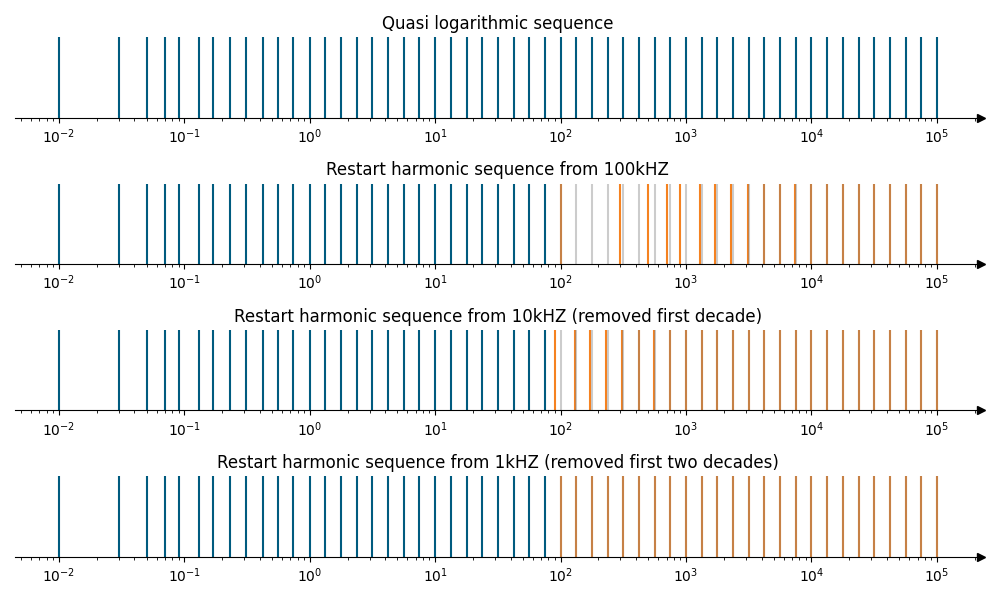
\includegraphics[width=1\linewidth]{figures/harmonics_supporting.png}
    \caption{Enter Caption}
    \label{fig:splitting_design}
\end{figure}

To summarize, for a CCCV experiment for batteries, on channel of the generator would have loaded in memory two low band multisine waves, one optimized for chronoamperometry and the other from chronopotentiometry, and the other channel have loaded the two optimized high band mutisine waves.

The automatic switch of the multisine during electrochemical experiments as described before can still be done by DEISchannel for the case of combined multisine waves passing during initialization the object MultisineWaveCombined, also provided  in the package TrueFormAWG.

\section{Automation of the acquisition for batteries}

The potentiostat is used only for the electric control of the cell while not applying any perturbation while the waveform generator provides the multi-frequency excitation as well as the quasi-cyclic voltammetry pattern. 
The arbitrary waveforms are loaded manually to the device via a .arb file transferred via USB drive from the computer. How the .arb file is build?
This approach was the one I used for the first two applications (topic of the third and final part of the thesis) of the dynamic impedance for energy storage, also published as peer-review articles.

For the goal of the thesis of acquiring the dynamic impedance during the CCCV cycling of a battery the previously described approach is not enough. 
Two problems arise: the first is the huge amount of data streamed from the device to the computer to be saved into the RAM, limited to a few GB, and secondly the need to change the waveform for the excitation  during constant current (chronopotentiometry) or constant voltage (chronoamperometry) steps. 
To overcome this problem and automation routine is needed, but before going into it I shall unpack the two issues one at the time. 
Recarding the managment of the streamed signals the problem is to sample for a long time, in the scale of weeks or months, while acquiring at high frequency. 
Let's say that one choses a moderate sampling frequency of 50kHz while sampling a system escited with a miximum frequency of 10kHz, it means 50kSa per second are stored, equivalent to 355 MSa per hour that we can translate to about 4.3 GB per channel per hour. 
Even using systems with huge memory, only a few hours of acquisition would be possible, not weeks. 
The alternative is to store into the hard drive the sampled signlas before the RAM is filled up and without loss. 
One can decide a fixed ammount of points for the storage or execute the saving at the end of a technique (chronopotentiometry or chronoamperometry). 
Before commenting which of the two approaches are more suitable for the project, I must discuss the second of the issues mentioned above. 
The multisine, its design will be throughly eplained in a later chapter, is not just characterized by the frquency content but also its absolute and the relative amplitude of the sinusoidal components. 
The absolute amplitude is important for making the experiment itself, in the sense that for a chronoamperometry experiment the amplitude in volt of the excitation is the exact value applied on the cell. 
For a chronopotentiometry experiment instead, the signal in volt prodiced by the generator is converted to current passing though the measurement resistor. 
It is clear that the amplitude of the excitation must be changed when the running technique is a chronoamperometry or a chronopotentiometry. 
In addition, the relative amplitudes of the single sinusoidal components must be optimized (instead of being all equal) to the system. 
The method I prefer to use is to measure the impedance once experimentally and deduce its module to decide the relative amplitude of each sinusodial component such that the output has a certain amplitude for a good signal to noise ratio. 
In other words, if one follows the formula

$$
V_{output}(\omega _i) = |Z_{exp}(\omega _i)| \times I_{input}(\omega _i)
$$

can deduce the necessary current to obtain a certain oscillation in volt for each sinusodial component for the system under study. 
It is foundamental to note that the relative amplitude for a chronoamperometry experiment would be the rexiprocal of the one for a chronopotentiometry techinque to maintain the same signal to noise ratio. 
For this reason one should generate two different multisine with the two series of relative amplitude and then generate them during the correct technique using a suitable total multisine amplitude to perturb the system enough. 
It is indeed an art that require trail and error and a lot of time spent on looking at the peaks of the Discrete Fourier Transform for input and otuput.









\subsection{Software solution}

The work around for both the questions seems to be an automatic system that can, during the execution of the experiment, changed the excitation in the waveform generator remotely accordignly to the technique in execution and save the signals from the scope when a technique is finished. 
This simple idea hides the main technical complication of this work: having a computer program that workd with the generator and scope, and also monitors the execution of the sequence of techniques that forms an CCCV experiment.
The software that BioLogic provides EC-Lab is not ment for software automatino but can only send trigger analog signals to other device. 
It would solve the communication with the generator but not with the streaming software of the scope. 
Luckily, BioLogic do provide the API for the control of the instruments in multiple programming languages, including Python. 
The downside is that the API is not officially supported and it is vary primitive. 
Especially the data has to be streamed from the machine and converted manually in the user code, similarly to the code for the scope. 
So I decided to write a library for the control of the BioLogic workstation in Python with some specific requirements:
\begin{itemize}
    \item work in multi-threaded fashion to allow multiple channels from the same machine to work independently and each of them to communicate to the device without blocking execution;
    \item allow easy integration with other libraries to create flexible set-up;
    \item allow to construct the same experiment structure, i.e. sequence of technqiues, of EC-Lab to compare results from both.
    \item implement software limits for voltage and current that consider the average value of the quantity to compensate the oscillation of the multisine.
\end{itemize}

\subsection{Design principle}

The automation of the instruments compatible with multi-threading uses the design pattern of the worker object. 
A worker object execute operation inside a \emph{while True} block on a dedicated thread, and terminates with a pause of 1 second of less (with the sleep command) during which the main thread is allowed to execute the code of another worker object. 
The multi-threading standard library of Python is capable of automatically manage all the objects without user indication in the code (compare to the other library like asyncio).

Worker object has a propriety with the name \emph{running} that can be used from other object to check their status. 
This idea is at the base of all the library used to syncronize the electrochemical workstation, waveform generator and scope. 
It is important to notice that given the modularity of the apporach, it is possible to use different hardware to perform the experiment in the same manner, given the interface is similar (i.e. it has the same name of the methods that return the same objects).

% Multi-threaded objects can share memory in the form of memory buffer to avoid the well known problem of concurrency. Since all the mathematical operation in the Python code uses the library Numpy and its array type for storing the data it made sense to me to have a circular buffer with the type of Numpy array to work with. Unfortunately the only existing implementation on public repositories (NpCircularBuffer) was not updated to the current version of Numpy, therefore I made and published my own simple implementation of a one-dimensional circular buffer with the name npbuffer and used it across the library needed for this project.

\section{DEIStools: a Python application for dynamic impedance}
% Clear, but needs a structural explanation before diving into components.
% Use a block diagram (even ASCII) to anchor the explanation.
% Avoid too much focus on worker objects — describe functionality.
The previous sections introduced the ideas of automating the multi-sine switch, save acquired signals periodically and process the signals online. 
These tasks are performed for each of the active channel of a multichannel electrochemical workstation. The hart of the operation is a library with the name DEIStools that contains everything need to prepare the experiment, execute it, analyses the data and visualize the results.
It builds upon the separate libraries that interface with the three devices of the set-up using the same \emph{worker object} building block discussed before.
DEIStools provides the object DEISchannel that automate the measurement. 
The user provide to the class initialization the objects for the Channel of the electrochemical workstation, the generator and the scope, already connected and initialized. 
For the online processing of the signals, another object is provided by DEIStools called PicoCalculator, that has the name suggest, takes the PicoScope object and extend its functionality to perform the calculations on a block of data of a specific length (one can think of the concept of windowing of signal processing). 
To continue into the idea of modularity, the calculation is performed by the object BlockCalculator that receives as arguments of its method a numerically converted copy of the signals (from the ADC values), and performs with them the FFT-EIS and downsampling.
With this design, the processing can be personalized for new experiment without touching the rest of the code for automation. The calculation is, as well, performed on a dedicated thread while the PicoScope object keep receiving data from the device without interruption.

Finally, the sequence of multisine waveforms, their amplitude, sampling frequency and when to turn them on in the sequence of the experimetn is also managed by a convenient object MultisineWave that the user passes to DEISchannel.
The modularity is provided by the software design pattern of dependency injection. The object Channel of pyeclab, for the control of a workstation channel accept as attribute a function that is always execute at the end of a technique, that, for the case of DEISchannel, executes the saving of the downsampled signals and updates the multisine.

\subsection{Software limits}

When a multisine is applyed on top of the drift, it is difficult to determine when to stop the galvanostatic experiment. 
Generally batteries are cycled between an upper and lower voltage limit and the constant voltage step of the CCCV terminated on a lower limit for the current. 
The easiest approach is to add to the desired limit the amplitude of the oscillation, but this is not always known. 
In my approach, I implemented two options for avarage limits. 
One is included in the DEISchannel object and computes the average over a user-selected number of points from the sampling of the workstation (note: not the scope, so the signal is likely to contain strong aliasing). 
The other is performed by the PicoCalculator object that uses the value of the zero-frequency bin in the DFT already calculated for the processing of the data, sparing any further computation. In both cases, the user can specify as many software limits as desired, using the proper syntax.


\section{Data and metadata saving}
FAIR data are essential for makeing the diffusion of DEIS possible.

% \section{The computation of impedance for non-stationary systems}
% %Under which conditions the system can be approximated as locally LTI
% %Over what window the drift is negligible
% %Why the multisine period must be shorter than the drift timescale

% \section{Online processing and data reduction} 
% \label{On-line computation}
% % This is central and should be highlighted earlier.
% % Add a conceptual figure
% The automation of the acquisition allow to record signals for battery cycling and mixed techniques but still has on other limitation regarding the data size. When considering the impedance of a battery, the desired frequency range might differ depending on the chemistry. In some cases 100Hz could be the maximum needed frequency for bigger batteries in pouch format, but when going to smaller sizes and laboratory scales it is generally needed to probe until higher frequency, up to 1MHz where the inductance of the connections cell to instrument became the predominant response (here I am not including solid state electrolytes that might need frequencies up to 7 MHz). For the application presented later, I determined an highest frequency of excitation of 100kHz (maintaining the lowest to 10mHz) that requires a sampling frequency of 500kHz or 1MHz (both worked in my tests using the following method, although according to the Nyquist limit 250kHz is enough). Such an high sampling rate would store very big data in the hard drive that soon will require expansion after weeks of measurement and experiment repetiotion. Furthermore the highest frequency would be repeated for a huge amount of times while we are actually interested of sampling long times to identify the lowest frequency. The upper part of the frequency band can be considered in a quasi-stationary condition and therefor doesn't require mathematical techniques to decouple with the main drift. The method used here follow this idea: calculating the impedance of the upper part of the frequency band (ex. above 10Hz) using the FFT-EIS method, apply a low-pass filter to remove these same frequencies and decimate the signal to a much lower rate (ex. 50Hz) to be stored for later estimation of the time-varying impedance (ex. with DMFA). Finally, the total spectra is reconstructed concatenating the impedance estimated with the two methods.

% This is the first contribution of this work: measuring broad-band non-stationary impedance continuously during the cycling of the battery.


% \section{Impedance estimation}
% % Good technical detail, but DMFA theory is misplaced.
% % Move DMFA theory to the identification chapter, keep practical aspects here.
% In the experimental works presented in this thesis, we estimated the impedance using the methods of the sliding short-time Fourier transform and dynamic multifrequency analysis; the first only during the online signal processing. The STFFT method has not much tuning. The only user parameters are the length of the window and the windowing function type. The length is dictated by the resolution that one wants to achieve, so on the lowest frequency component of the excitation. The windowing function instead alters the input and output signals time series to put more or less importance to the central part of the signal rather than the borders (makes the impedance confined in time at the price of spectral power) to obtain the instantaneous impedance at the middle points. For the experiment presented here, I assumed that being the drift of the system much slower than the perturbation, the impedance would not vary much and no windowing function is necessary. For the Dynamic Multi-Frequency Analysis, one needs to chose a filter function with care. Here we used the symmetric Fermi-Dirac delta with bandwidth of 0.01 Hz and an order of 8. A previous publication of the group showed the effect of these two parameters on the final result. The most important is the bandwidth because it reflects on the number of spectra estimated and their separation in time. Battistel and al. showed in XX the shape of the filter function when trasnformed to the time domain and it is similar to a sinc function for its main lobe and small oscillation asintothycally to zero. The dynamic multifrequency analysis performes a multiplication in the frequency domain  of the filter with the fourier spectra of the signal around one frequency, that correspond to a convolution of the time domain. Hence the time-domain transformed filter as a function shifted in time by a quantity equal to the reciprocal of the bandwidth. The windows should not be shorter than the period of the multisine and furthermore one should put care in the oscillating lobes that could bias the impedance estimation, as shown in Chukwu.

% In both methods, one can strongly reduce the zero-frequency skirt in the Fourier space and the Gibbs effect  by removing the baseline for current and voltage signals. I chose to use just a simple baseline removing because other classical methods did not work for me. Typically one can use sliding window averaging, spline or polynomial fitting or gaussian process regression to name the main one. In my experience non of these methods could effectively decouple the trend and the first few frequencies of the multisine that are overlapping. A complete Python library can be used to test these and more trend removal techniques, it is called Wotan. Hellemans and al. developed a method for de-trending signals with low frequency containing multi-sine but there is no available Python implementation to try out and the functional analysis used in the official is above my mathematical skills to implementing it myself.

% \section{Consideration on the drift}
% % Why using quasi cyclic voltammetry.

\section{Limitations and future improvements}
% Expensive hardware, could be streamlined
% Clock synchronization of generator and sampler
% Better optimization of the multisine